\documentclass[tikz,convert={density=300,outext=.png}]{standalone}
\usetikzlibrary{calc}

\begin{document}
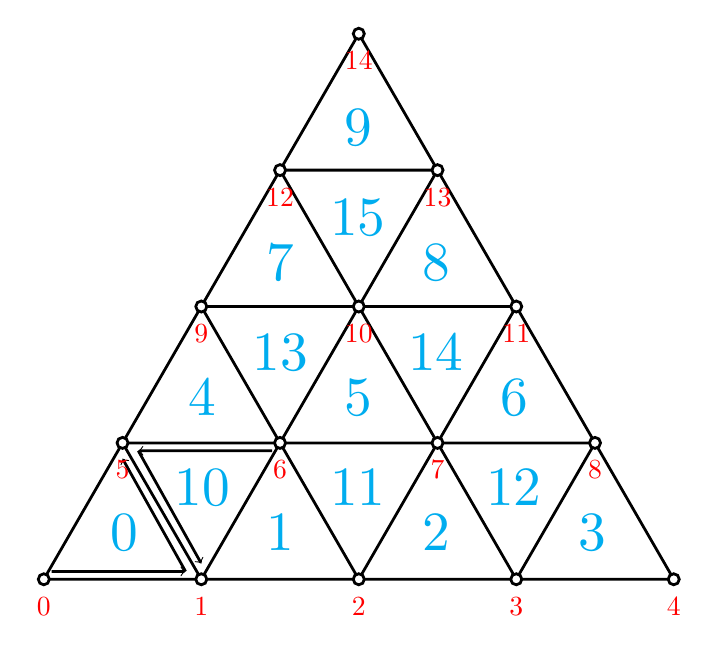
\begin{tikzpicture}[transparency group=knockout]
\coordinate (dx) at (2,0);
\coordinate (dy) at (0,2);
\coordinate (a7) at ($0.866*(dy)-0.5*(dx)$);
\coordinate (a8) at ($(a7)+(dx)$);
\coordinate (a3) at ($-1*(dx)$);
\coordinate (a5) at ($-1*(a3)$);
\coordinate (a4) at ($0.5*(a3)+0.5*(a5)$);
\coordinate (a0) at ($(a7)-2*0.866*(dy)$);
\coordinate (a1) at ($(a0)+(dx)$);
\coordinate (a2) at ($(a1)+(dx)$);
\coordinate (a6) at ($(a5)+(dx)$);
\coordinate (a9) at ($(a8)+(dx)$);
\coordinate (a10) at ($(a4)+2*0.866*(dy)$);
\coordinate (a11) at ($(a10)+(dx)$);
\coordinate (a12) at ($(a3)+(a3)-(a7)$);
\coordinate (a13) at ($(a10)+(a10)-(a7)$);
\coordinate (a14) at ($(a6)+(a6)-(a9)$);

\coordinate (a9) at ($0.866*(dy)-0.5*(dx)$);
\coordinate (a10) at ($(a9)+(dx)$);
\coordinate (a5) at ($-1*(dx)$);
\coordinate (a7) at ($-1*(a5)$);
\coordinate (a6) at ($0.5*(a5)+0.5*(a7)$);
\coordinate (a1) at ($(a9)-2*0.866*(dy)$);
\coordinate (a2) at ($(a1)+(dx)$);
\coordinate (a3) at ($(a2)+(dx)$);
\coordinate (a8) at ($(a7)+(dx)$);
\coordinate (a11) at ($(a10)+(dx)$);
\coordinate (a12) at ($(a6)+2*0.866*(dy)$);
\coordinate (a13) at ($(a12)+(dx)$);
\coordinate (a0) at ($(a5)+(a5)-(a9)$);
\coordinate (a14) at ($(a12)+(a12)-(a9)$);
\coordinate (a4) at ($(a8)+(a8)-(a11)$);

\draw (a0) -- (a4) (a5) -- (a8) (a9) -- (a11) (a12) -- (a13);
\draw (a0) -- (a14) (a1) -- (a13) (a2) -- (a11) (a3) -- (a8);
\draw (a5) -- (a1) (a9) -- (a2) (a12) -- (a3) (a14) -- (a4);

\draw[->] ($(a0)+0.05*(dy)+0.05*(dx)$) -- ($(a1)+0.05*(dy)-0.1*(dx)$);
\draw[->] ($(a1)+0.05*(dy)-0.1*(dx)$) -- ($(a5)-0.1*(dy)$);

\draw[->] ($(a6)-0.05*(dy)-0.05*(dx)$) -- ($(a5)-0.05*(dy)+0.1*(dx)$);
\draw[->] ($(a5)-0.05*(dy)+0.1*(dx)$) -- ($(a1)+0.1*(dy)$);

\node[below=3pt,fill,opacity=0,text opacity=1,color=red] at (a0) {0};
\node[below=3pt,fill,opacity=0,text opacity=1,color=red] at (a1) {1};
\node[below=3pt,fill,opacity=0,text opacity=1,color=red] at (a2) {2};
\node[below=3pt,fill,opacity=0,text opacity=1,color=red] at (a3) {3};
\node[below=3pt,fill,opacity=0,text opacity=1,color=red] at (a4) {4};
\node[below=3pt,fill,opacity=0,text opacity=1,color=red] at (a5) {5};
\node[below=3pt,fill,opacity=0,text opacity=1,color=red] at (a6) {6};
\node[below=3pt,fill,opacity=0,text opacity=1,color=red] at (a7) {7};
\node[below=3pt,fill,opacity=0,text opacity=1,color=red] at (a8) {8};
\node[below=3pt,fill,opacity=0,text opacity=1,color=red] at (a9) {9};
\node[below=3pt,fill,opacity=0,text opacity=1,color=red] at (a10) {10};
\node[below=3pt,fill,opacity=0,text opacity=1,color=red] at (a11) {11};
\node[below=3pt,fill,opacity=0,text opacity=1,color=red] at (a12) {12};
\node[below=3pt,fill,opacity=0,text opacity=1,color=red] at (a13) {13};
\node[below=3pt,fill,opacity=0,text opacity=1,color=red] at (a14) {14};

\node[scale=2,color=cyan] at ($0.33*(a0)+0.33*(a1)+0.33*(a5)$) {0};
\node[scale=2,color=cyan] at ($0.33*(a1)+0.33*(a2)+0.33*(a6)$) {1};
\node[scale=2,color=cyan] at ($0.33*(a2)+0.33*(a3)+0.33*(a7)$) {2};
\node[scale=2,color=cyan] at ($0.33*(a3)+0.33*(a4)+0.33*(a8)$) {3};
\node[scale=2,color=cyan] at ($0.33*(a5)+0.33*(a6)+0.33*(a9)$) {4};
\node[scale=2,color=cyan] at ($0.33*(a6)+0.33*(a7)+0.33*(a10)$) {5};
\node[scale=2,color=cyan] at ($0.33*(a7)+0.33*(a8)+0.33*(a11)$) {6};
\node[scale=2,color=cyan] at ($0.33*(a9)+0.33*(a10)+0.33*(a12)$) {7};
\node[scale=2,color=cyan] at ($0.33*(a10)+0.33*(a11)+0.33*(a13)$) {8};
\node[scale=2,color=cyan] at ($0.33*(a12)+0.33*(a13)+0.33*(a14)$) {9};

\node[scale=2,color=cyan] at ($0.33*(a6)+0.33*(a5)+0.33*(a1)$) {10};
\node[scale=2,color=cyan] at ($0.33*(a7)+0.33*(a6)+0.33*(a2)$) {11};
\node[scale=2,color=cyan] at ($0.33*(a8)+0.33*(a7)+0.33*(a3)$) {12};
\node[scale=2,color=cyan] at ($0.33*(a10)+0.33*(a9)+0.33*(a6)$) {13};
\node[scale=2,color=cyan] at ($0.33*(a11)+0.33*(a10)+0.33*(a7)$) {14};
\node[scale=2,color=cyan] at ($0.33*(a13)+0.33*(a12)+0.33*(a10)$) {15};

\draw[fill=white] (a0) circle(2pt); 
\draw[fill=white] (a1) circle(2pt);
\draw[fill=white] (a2) circle(2pt);
\draw[fill=white] (a3) circle(2pt); 
\draw[fill=white] (a4) circle(2pt); 
\draw[fill=white] (a5) circle(2pt); 
\draw[fill=white] (a6) circle(2pt); 
\draw[fill=white] (a7) circle(2pt); 
\draw[fill=white] (a8) circle(2pt); 
\draw[fill=white] (a9) circle(2pt); 
\draw[fill=white] (a10) circle(2pt); 
\draw[fill=white] (a11) circle(2pt); 
\draw[fill=white] (a12) circle(2pt); 
\draw[fill=white] (a13) circle(2pt); 
\draw[fill=white] (a14) circle(2pt); 

\end{tikzpicture}
\end{document}
